\section{Experiments and Results}
Present simulation results, analysis, and performance comparisons. 
Figure example (Fig~\ref{F:test-a}).
Table example (Table~\ref{table}).

\begin{figure}[htb]
    \centering
    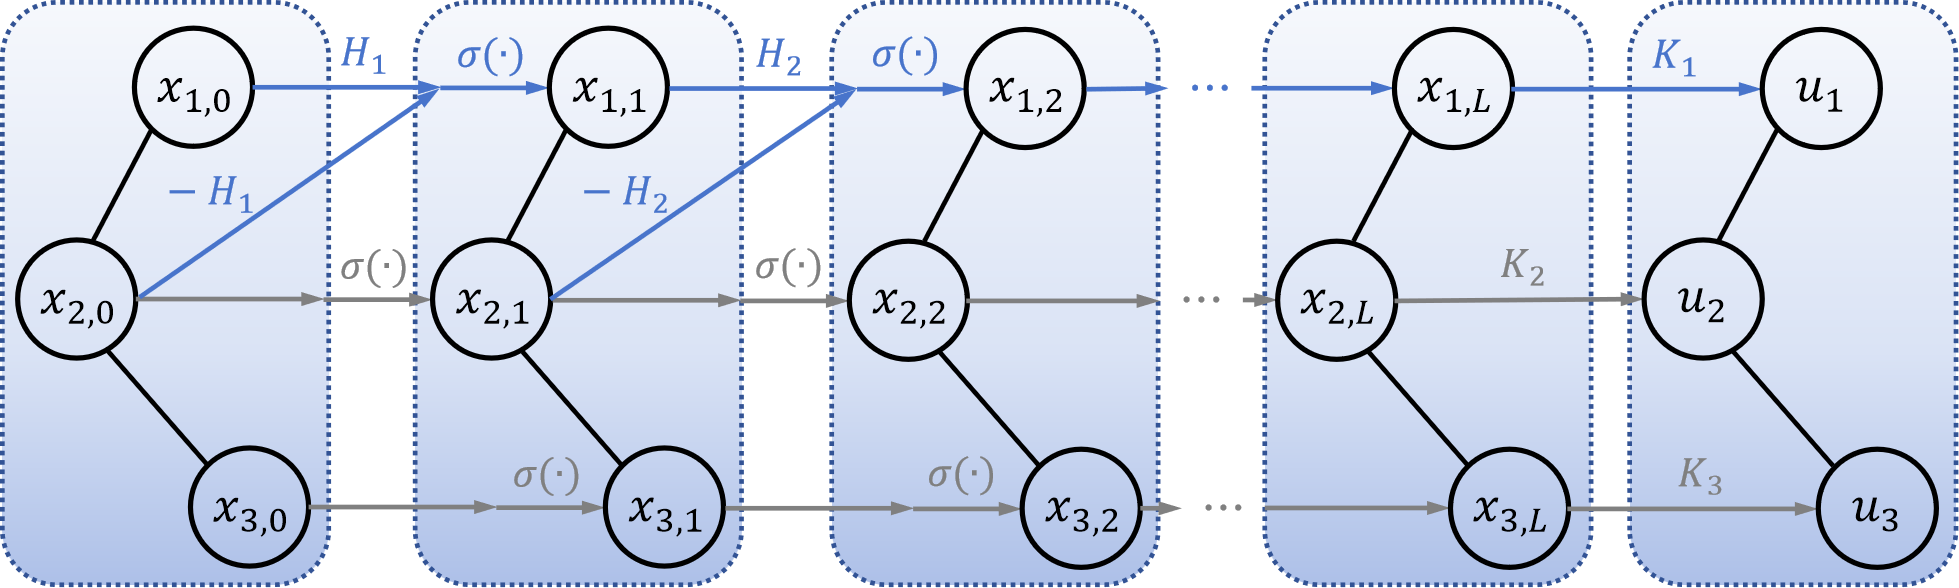
\includegraphics[width=.5\textwidth]{Images/example.png}
    \caption{Test image}
    \label{F:test-a}
\end{figure}

\begin{figure}[htb]
    \centering
    \begin{subfigure}[t]{.45\linewidth}
        \centering
        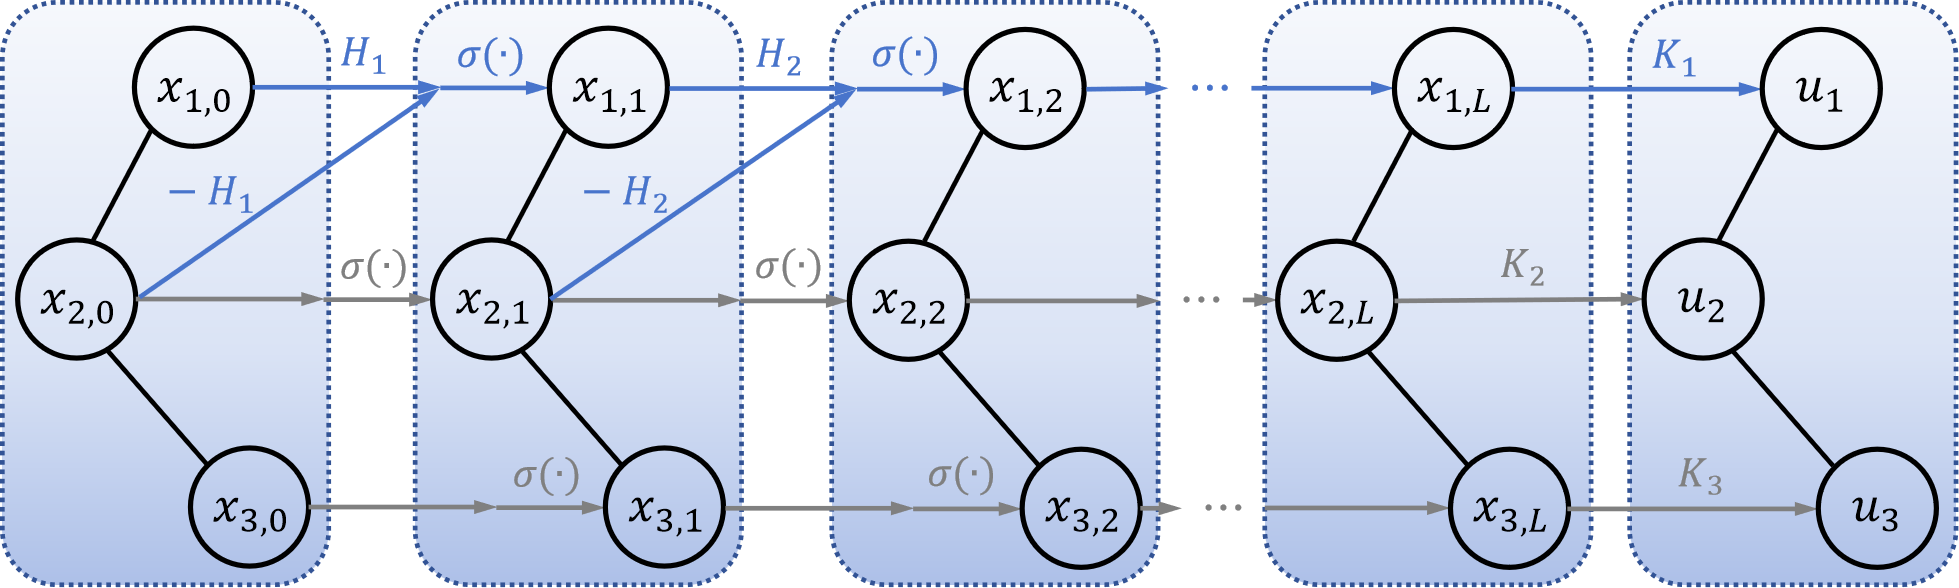
\includegraphics[width=1\textwidth]{Images/example.png}
        \caption{Test image 1}
        \label{F:test-b-sub-a}
    \end{subfigure}
    \hfill
    \begin{subfigure}[t]{.45\linewidth}
        \centering
        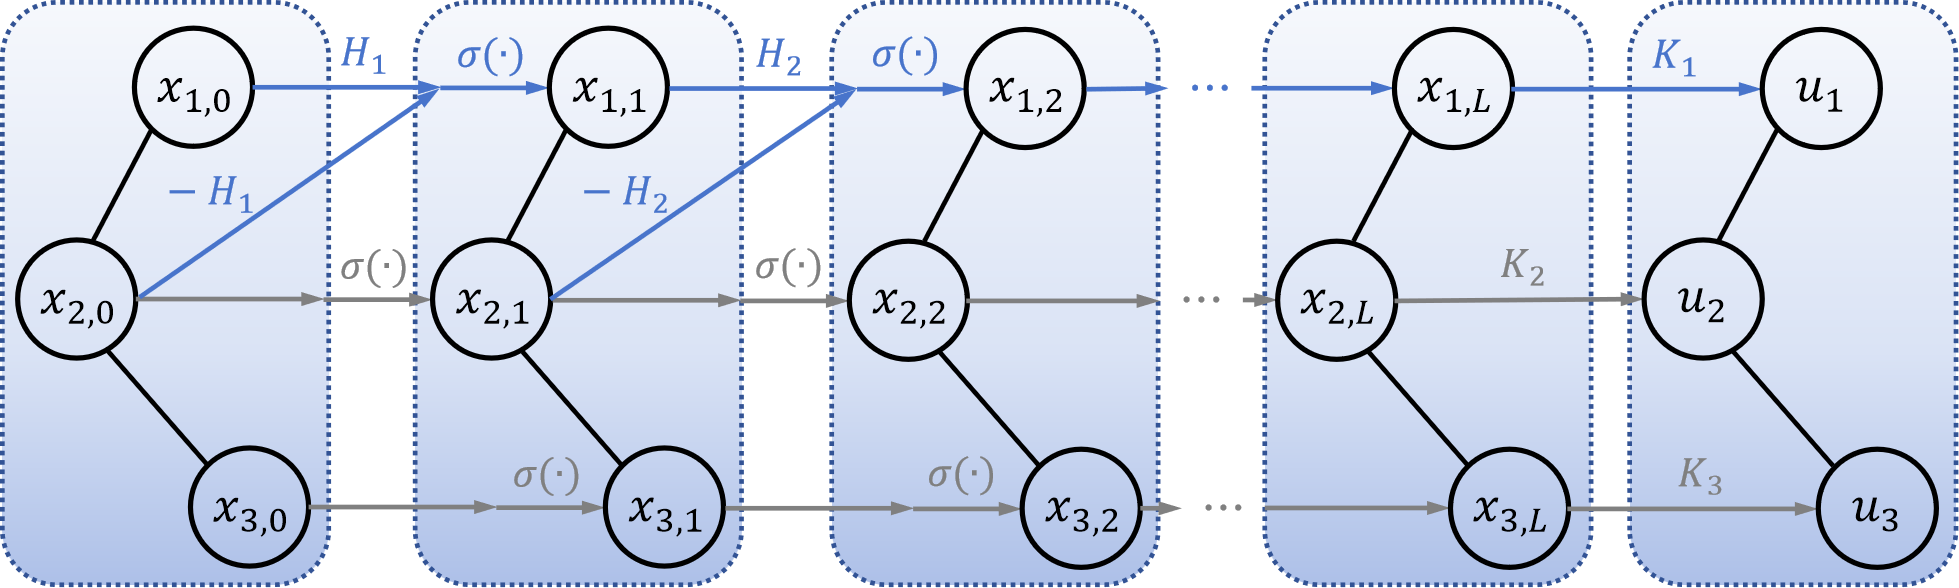
\includegraphics[width=1\textwidth]{Images/example.png}
        \caption{Test image 2}
        \label{F:test-b-sub-b}
    \end{subfigure}
    \caption{Test subimages}
    \label{F:test-b}
\end{figure}

\begin{table}[htb]  % h-here,t-top,b-bottom,优先级依次下降
    \settablefont
    \caption{Table caption}
    \label{table}
    \begin{tabular}{lc} % 三线表不能有竖线,l-left,c-center,r-right
        \toprule  % 三线表-顶线
        Example    &   Result \\
        \midrule  % 三线表-中线
        Example1   &   0.25 \\
        Example2   &   0.36 \\
        \bottomrule   % 三线表-底线
    \end{tabular}  % 续表用longtable代替tabular
\end{table}

